\chapter{Az alkalmazás implementációja}
\section{C\# implementáció}
% Meg kellene mutatni, hogy milyen API és újrahasznosítható elemek készültek el.
Az alkalmazás implementációja során fontos volt a C\# alapelveinek betartása (OOP elvek és nyelv specifikus elvek együttvéve). Szerencsére nem kellett újra feltalálni semmit, hisz a .NET rendelkezik gráf rajzolóval, megjelenítővel, (hozzá különféle szolgáltatásokkal) és különféle standard formátumú fileokra készített feldolgozó modulokkal. Ebből adódóan a lényeges munka az átalakító modulok és az adatstruktúrák megírása volt. 
\begin{cpp}
internal class Model
    {
        public class Net
        {
            public List<Place> Places { get; set; }
            public List<Transition> Transitions { get; set; }
            public List<Arc> Arcs { get; set; }

            public Net()
            {
                Places = new List<Place>();
                Transitions = new List<Transition>();
                Arcs = new List<Arc>();
            }
        }

        public class Node
        {
            public string Label { get; set; }
        }

        public class Place : Node
        {
            public List<Token> Tokens { get; set; }
        }

        public class Transition : Node
        {

        }
        public class Arc
        {
            public Node Input { get; private set; }
            public Node Output { get; private set; }
            public int Multiplicity { get; set; }
        }

        public class Token
        {
            public string Color { get; set; }
        }
    }
\end{cpp}
\textsl{A Színezett Petri-háló adatstruktúrája}

A step-by-step animáció úgy készül, hogy a megfelelő lépések legenerálódnak. A képek bekerülnek egy pipe-ba, ami a program beállításaiban megadott időzítő ütemére átadásra kerülnek megjelenítésre. 
A lépések addig számítódnak amíg a folyamat teljes egészében lefut, vagy egy olyan nodehoz nem ér ami felhasználói bevitelt vár. Ekkor a számítás szünetel és a UI megjelenítő előkészít egy input mezőt. Az input mező a felhasználói adatbevitel után (ha nem szükséges a következő lépéshez) eltűnik, az átláthatóság kedvéért. A mező tartalma átkerül feldolgozásra és általában token formájában kerül megjelenítésre. (Előfordulhat, hogy a program egy várakozási időt kér. Ez esetben is megjelenítődik token formájában, de a lényeg, a háló tranziciói csak egy bizonyos idő (feldolgozási-ciklusidő) függvényében tüzelnek. Az alkalmazásban nem volt szempont a konvertált hálók mentése, de könnyűszerrel megoldható.

Az alkalmazás megnyitásakor egy helyfoglaló kép, és az alkalmazás kezdeti állapotú vezérlőfelülete fogad. 
\begin{figure}[h!]
\centering
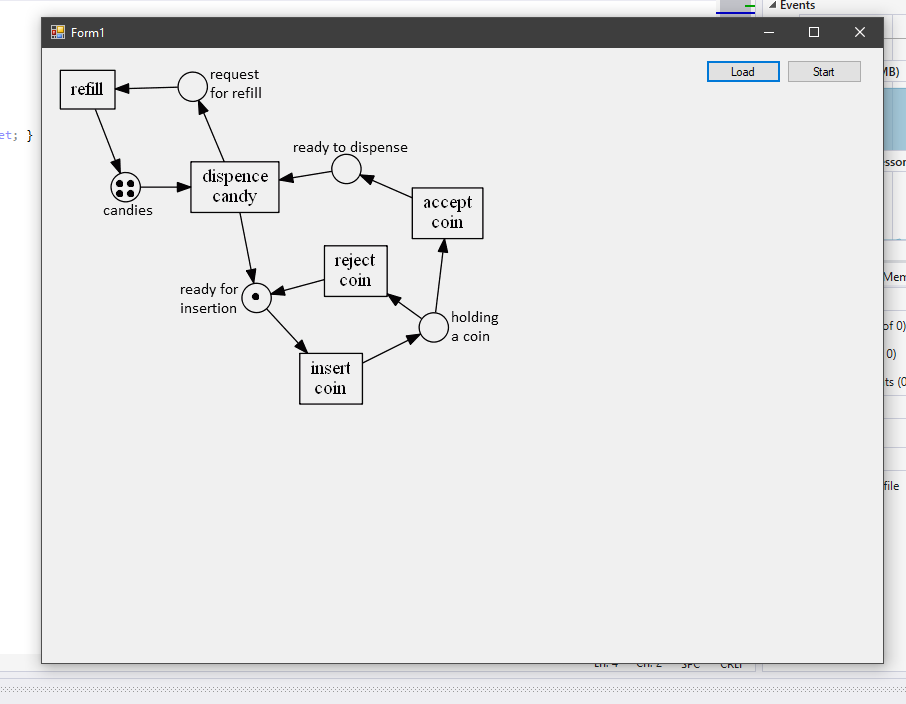
\includegraphics[scale=0.5]{images/UIlayout.png}
\caption{Az alkalmazás kezdeti állapota:}
\label{fig:flow}
\end{figure}
A vezérlőfelület két gombot tartalmaz alapállásban. Egy load és egy start gombot. A load gomb segítségével egy BPEL file tallózható, míg a start a file kiválasztása  után indítja a konverziós és szimulációs szubrutinokat. 
\begin{figure}[h!]
\centering
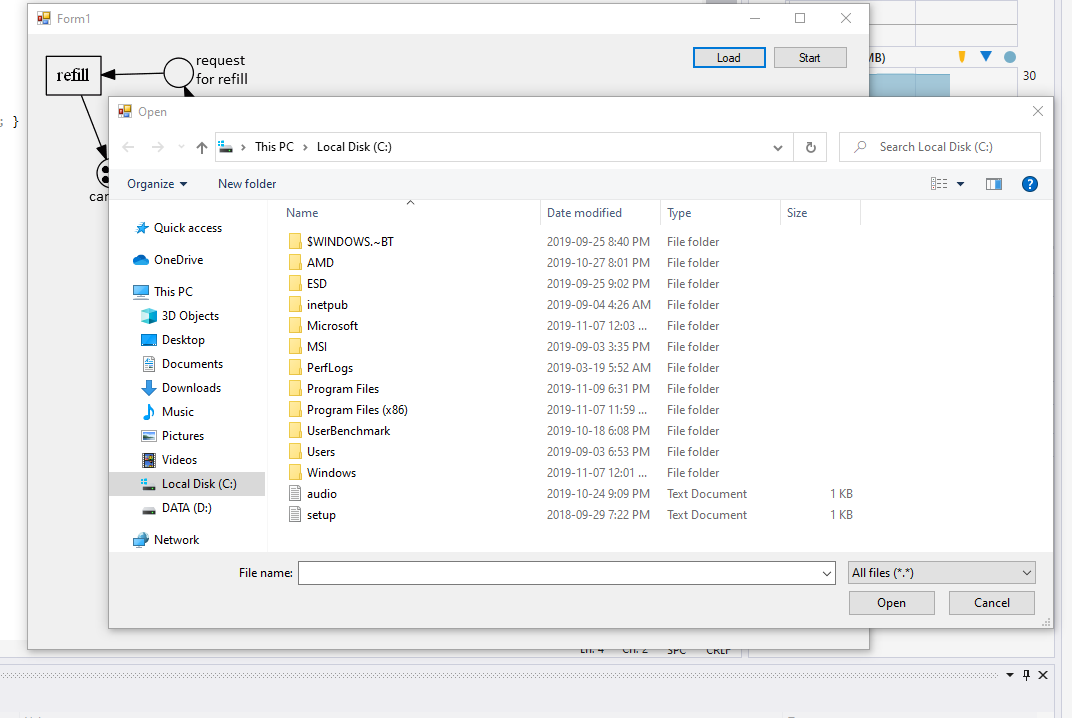
\includegraphics[scale=0.5]{images/fileDialog.png}
\caption{Az alkalmazás tallózó ablaka}
\end{figure}

A tesztelés során szükségessé vált a beolvasott file kiíratása, ezért DEBUG üzemmód esetén a beolvasott file a képernyőre kerül egy MessageBox tartalmaként.
\begin{figure}[h!]
\centering
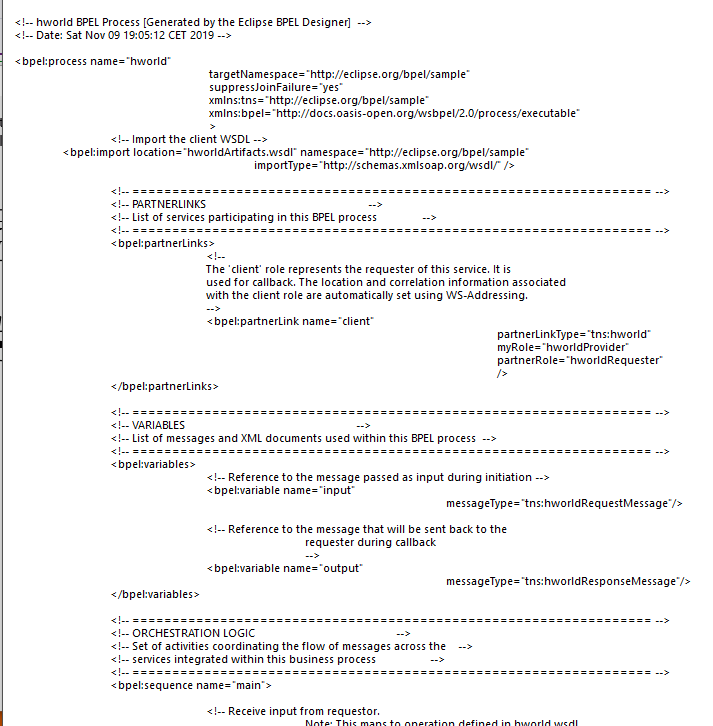
\includegraphics[scale=0.4]{images/debug.png}
\caption{Az alkalmazás debug üzenete}
\end{figure}

Ha a konverzió sikeres akkor a megjelenítőbe kerül a fordított folyamat, ha nem akkor az alkalmazás üzenttel jelzi a konverziós hibát. Sikeres futás után az alkalmazás vissza áll STOP állapotba.
\begin{figure}[h!]
\centering
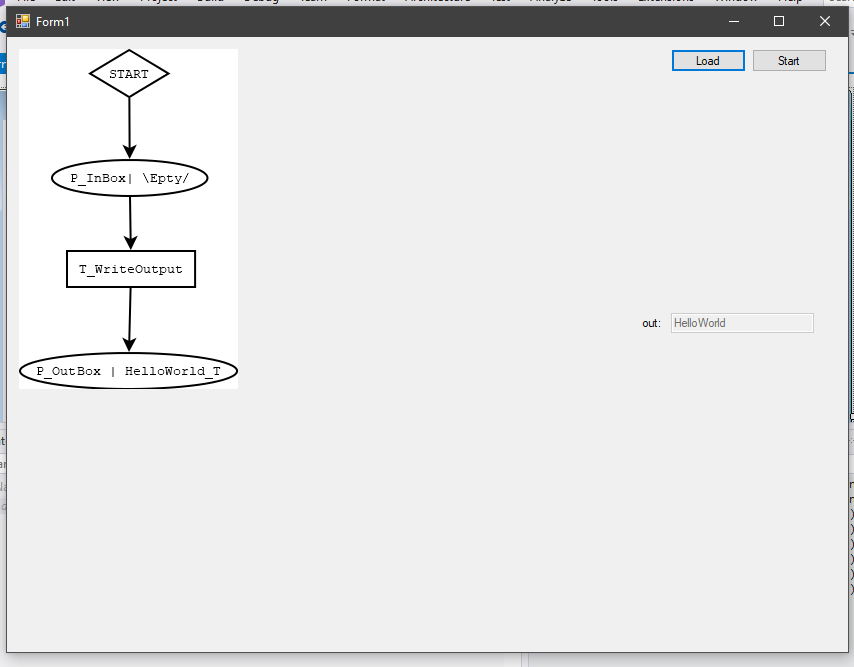
\includegraphics[scale=0.4]{images/done.png}
\caption{Az alkalmazás szimuláció végi állapota}
\end{figure}
\newpage
\section{Python implementáció}
A dolgozatban két programozási nyelvet használtam, ami az alábbiakkal indokolható. Az első hogy, a dolgozat kezdeti szakaszán még csak a modellezésre gondoltam, és ezért egy olyan nyelvet választottam ami konverziós és automatizálási lehetőségekben gazdag, mindemellett hatékony és gyors is, valamint már tapasztaltabban alkalmazom. Így esett a választás a C\# -ra. A dolgozat későbbi fejezetében tárgyalom a validáció számítást, ami optimalizáló algoritmust használ. Ez a funkció később merült fel a projektben. Kezdetben az is C\# nyelven lesz implementálva. Később komplikáció adódott, ami a második indok; A C\# , ugyanis főleg nagyvállalati termelésre szánt programnyelv, nem kutatási célokra készült. Ez a gyakorlatban azt jelenti, hogy bár LP feladatot lehet vele megoldani, nem rendelkezik megfelelő (ingyenes, vagy kényelmesen alkalmazható) LP feladatmegoldó könyvtárral. Ekkor került a fókusz a mára általánossá vált adatmodellezési, és kutatási nyelvre, a Pythonra. A Python PuLP csomagja egy LP feladat megoldó csomag, ami rendelkezik előregyártott parametrizálásra kész szubrutinokkal és struktúrákkal, amik megkönnyítik az LP megoldásokat. A megoldás egyenes úton előáll és nem kell extra műveletek sokaságát végezni. A nyelv egyszerűsége miatt a Python nem szült különösebb problémákat. A két modul kommunikációja megoldható egy kapcsolattartó modullal vagy rendszerhívásokkal.

\section{Tesztelés, tapasztalatok}
% Itt kifejezetten az alkalmazás szemszögéből (nem pedig üzleti folyamatokra vonatkozóan) kellene bemutatni az alkalmazást.
A megjelenítéskor probléma lehet a gép számítási kapacitása, vagy annak kihasználhatatlansága. Tesztelés során nagy méretű hálók generálása során, a rajzfolyamat elhúzódhat, ez azt eredményezi, hogy a megjelenítéskor az animáció lassabb lesz, mert a megjelenítő szubrutin a képek elkészülésére vár. A lassulási probléma valamilyen szinten kiküszöbölhető a program aszinkron, több szálú futtatásával, de ekkor ügyelni kell arra, hogy az így generált képek megfelelő sorrendben legyenek pipeolva a megjelenítő számára. (Mivel a két tesztgépen nem volt értelme a többszálú futtatásnak, ezért kivételre került. Az első gépen a processzor egy magja csak több ezer node esetén kezdett lassabban dolgozni, a második gépen a 2 mag pedig nem hozott számottevő javulást.)

A teszteket nehezítette, hogy nem mindig lehetséges kölcsönös, egyértelmű leképzés, ezért a képzési szabályok se adódtak triviálisan. Ezekről alapos kivizsgálással lehetett csak meggyőződni, hogy valóban helyes eredményt produkálnak. További nehezítő körülmény, (bár nem képzi a dolgozat törzs szoftveres részét) a különböző szükséges BPEL teszt szerverek megléte. A Microsoft biztosít BizTalk 2010es kiadású teszt szervert fejlesztésre, de ez szigorúan Hyper-V virtuális gépen futtatható. (Magáért a tényleges szerver szoftverért csak mint cég/vállalkozás lehet teszt licencet igényelni. Továbbá a Microsoft nem folytatja BizTalk szerverhez tartozó jelentős frissítések fejlesztését, és jelenleg nem tervezi új szerver kiadását sem.) A másik alternatíva, a szabadon elérhető Apcahe ODE szerver. Ennek beüzemelése egy JAVA virtuális géppel kezdődik. Erre épül egy Apache TomCat szerver, ami ténylegesen az ODE környezetet tudja biztosítani. Ez az együttállás azt eredményezi, hogy bármelyik modul enyhe hibája egy láncreakciót indíthat, ami ugyan engedi a szervert futni, de tényleges használata nem lehetséges ilyenkor. További érdekesség, hogy a portokon rendszerint fennakad, azaz ha osztozni kell egy porton (pl 8080) még ha az nincs jelenleg használva, de (Windows rendszerben lehet előre foglalni, ilyenkor) valamelyik program igényelheti, hiába akadályozza a Windows a portok egymásra definícióját  az ODE nem működik vagy ép JAVA runtime errort ad ami nincs rendesen dokumentálva vagy timeout hosszú ideig várakozik, aztán hibakóddal leáll. 
